\section{Grounding the Evaluation: The Gain Is Invisible to a VLM}
\label{sec:grounded_eval}

The visual modalities expose the symmetric half of the framework (P3): even when grounded feedback \emph{does} fix the artifact, an ungrounded metric cannot see it.

\paragraph{The default VLM judge is structurally blind.} Our starting evaluator is a binary per-requirement rubric scored by a VLM over a screenshot. On $15$ dense academic-paper architecture figures, even with native-resolution quadrant tiling, this judge rates \textbf{$14$ of $15$} single-shot renders ``perfect'', i.e.\ satisfying every \emph{content} requirement it is asked to check (the right components present, labels correct). Layout geometry is simply not a question the screenshot lets it answer. By direct inspection the renders are broken (superimposed section titles, labels spilling out of boxes), so the failure is mechanical, not fixable by prompting the judge better. Screenshots are captured at $1080$\,px, so any content overflowing the canvas is cropped \emph{off-frame before the image reaches the judge} (the defect is literally absent from the pixels the model sees), and small in-frame overlaps fall below its acuity. A deterministic DOM-geometry check finds only \textbf{$3$ of $15$} are actually clean. The $14$-vs-$3$ gap is therefore not a \emph{wrong} answer to the same question but the judge being \emph{structurally unable to observe} the property that matters (\Cref{fig:blind}). (This initial probe is a deliberately hard, unconstrained set. The suite scored in \Cref{tab:geometric} is generated under the design-principle prompt of \Cref{sec:method} and is correspondingly cleaner single-shot, with headroom that is genuine task difficulty surviving a strong prompt, not a weak one.)

\begin{figure}[t]
\centering
\begin{subfigure}[b]{0.35\linewidth}
\centering
\begin{tikzpicture}
\begin{axis}[width=\linewidth,height=4.2cm,
  ybar,bar width=20pt,ymin=0,ymax=16,
  ylabel={\footnotesize figures rated clean (of 15)},
  symbolic x coords={VLM judge,DOM geom.},xtick={VLM judge,DOM geom.},
  xtick pos=bottom,ytick pos=left,
  enlarge x limits=0.55,nodes near coords,
  nodes near coords style={font=\footnotesize},
  ymajorgrids,ytick={0,5,10,15},
  every node near coord/.append style={anchor=south}]
  \addplot[draw=cSS!60!black,fill=cSS!35,bar shift=0pt] coordinates {(VLM judge,14)};
  \addplot[draw=cRV!60!black,fill=cRV!35,bar shift=0pt] coordinates {(DOM geom.,3)};
  \legend{}
\end{axis}
\end{tikzpicture}
\caption{The VLM passes $14/15$, the deterministic instrument only $3/15$.}
\label{fig:blind}
\end{subfigure}\hfill
\begin{subfigure}[b]{0.62\linewidth}
\centering
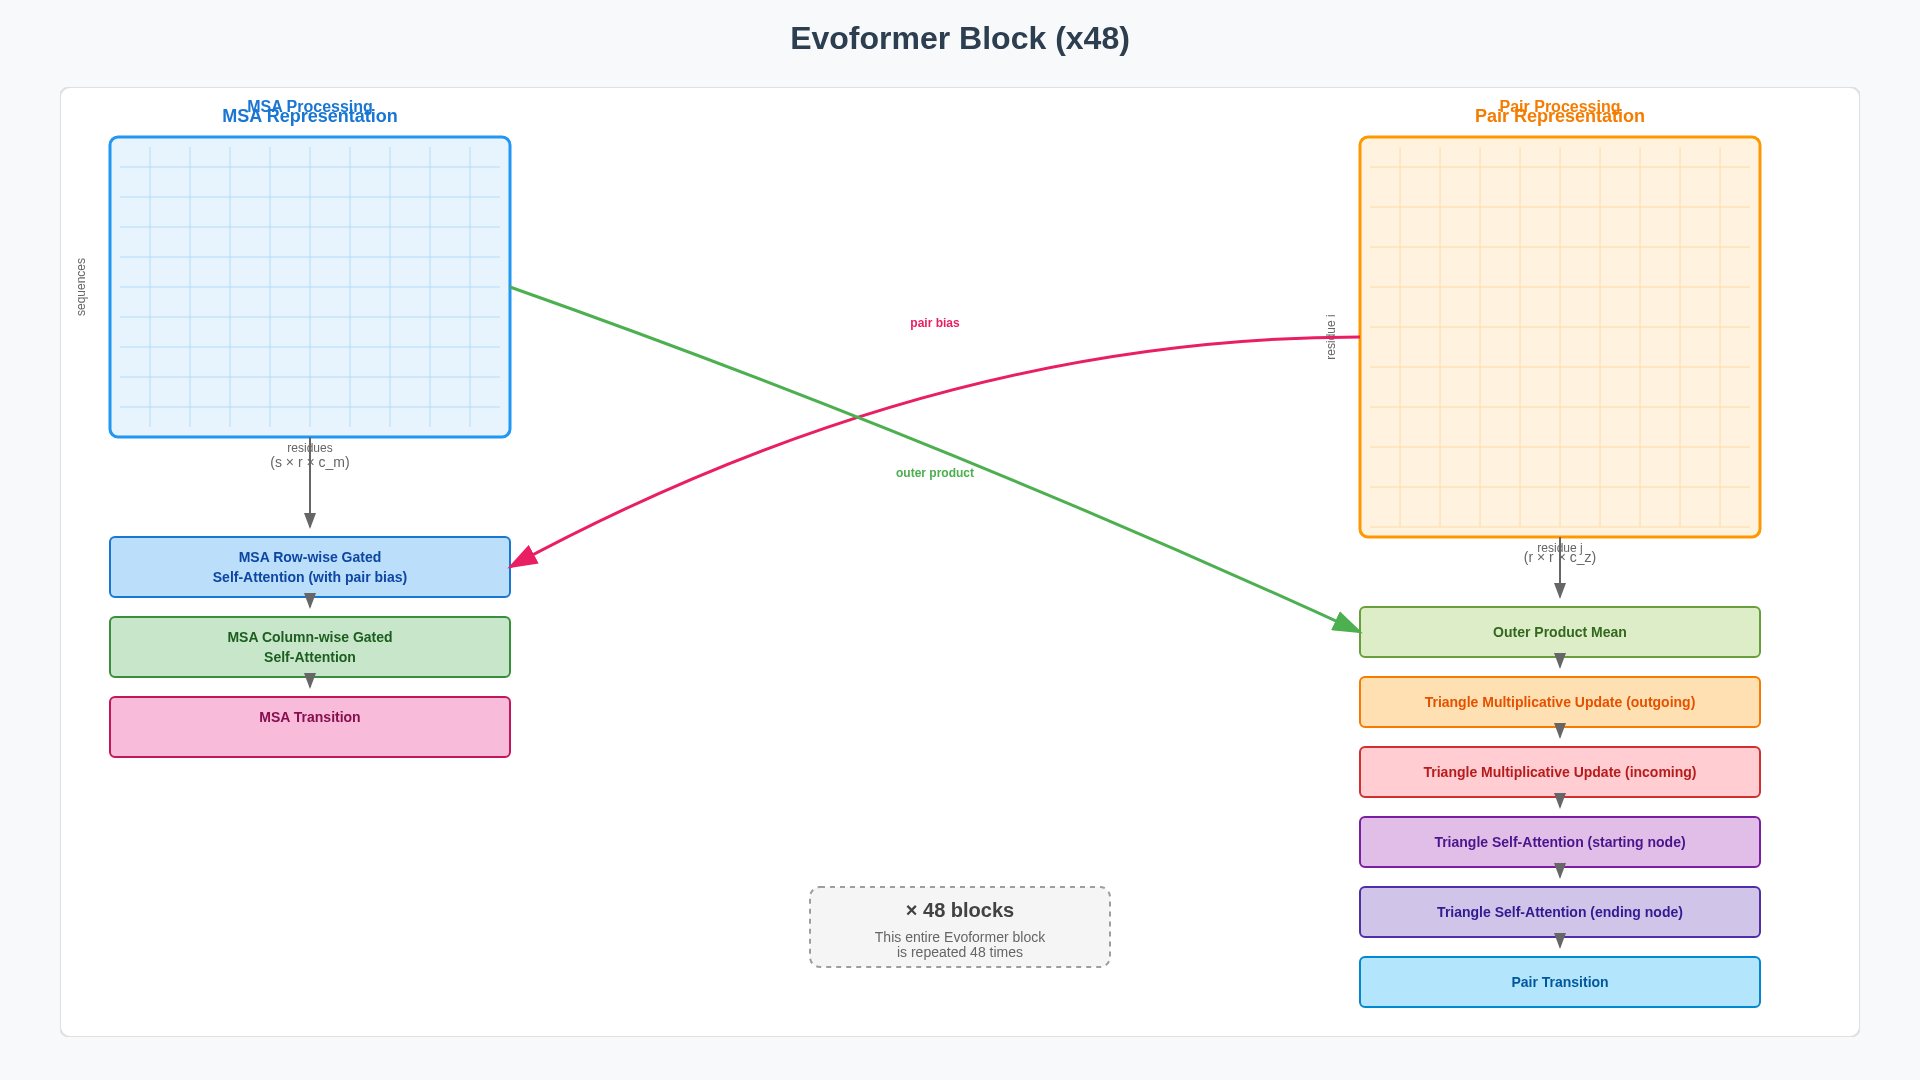
\includegraphics[width=\linewidth]{figures/evoformer_singleshot_vlm_perfect.png}
\caption{A single-shot figure the VLM rated ``perfect'': both section titles are superimposed (``MSA Processing'' over ``MSA Representation''; ``Pair Processing'' over ``Pair Representation'') and axis labels collide with the matrix borders.}
\label{fig:evoformer}
\end{subfigure}
\caption{\textbf{The default VLM judge is structurally blind to layout defects.} \textbf{(\subref{fig:blind})} On the same $15$ single-shot academic figures, the VLM-on-a-screenshot judge rates $14$ ``perfect'' while the deterministic DOM-geometry instrument finds only $3$ actually clean. The other $11$ are broken in ways cropped off-frame or below VLM acuity. \textbf{(\subref{fig:evoformer})} A representative ``perfect''-rated render whose text-on-text overlaps ($\ge6$\,px) are exactly what the geometry check flags and the screenshot judge misses.}
\label{fig:blindpair}
\end{figure}

\begin{figure}[t]
\centering
\begin{subfigure}[b]{0.49\linewidth}
\centering
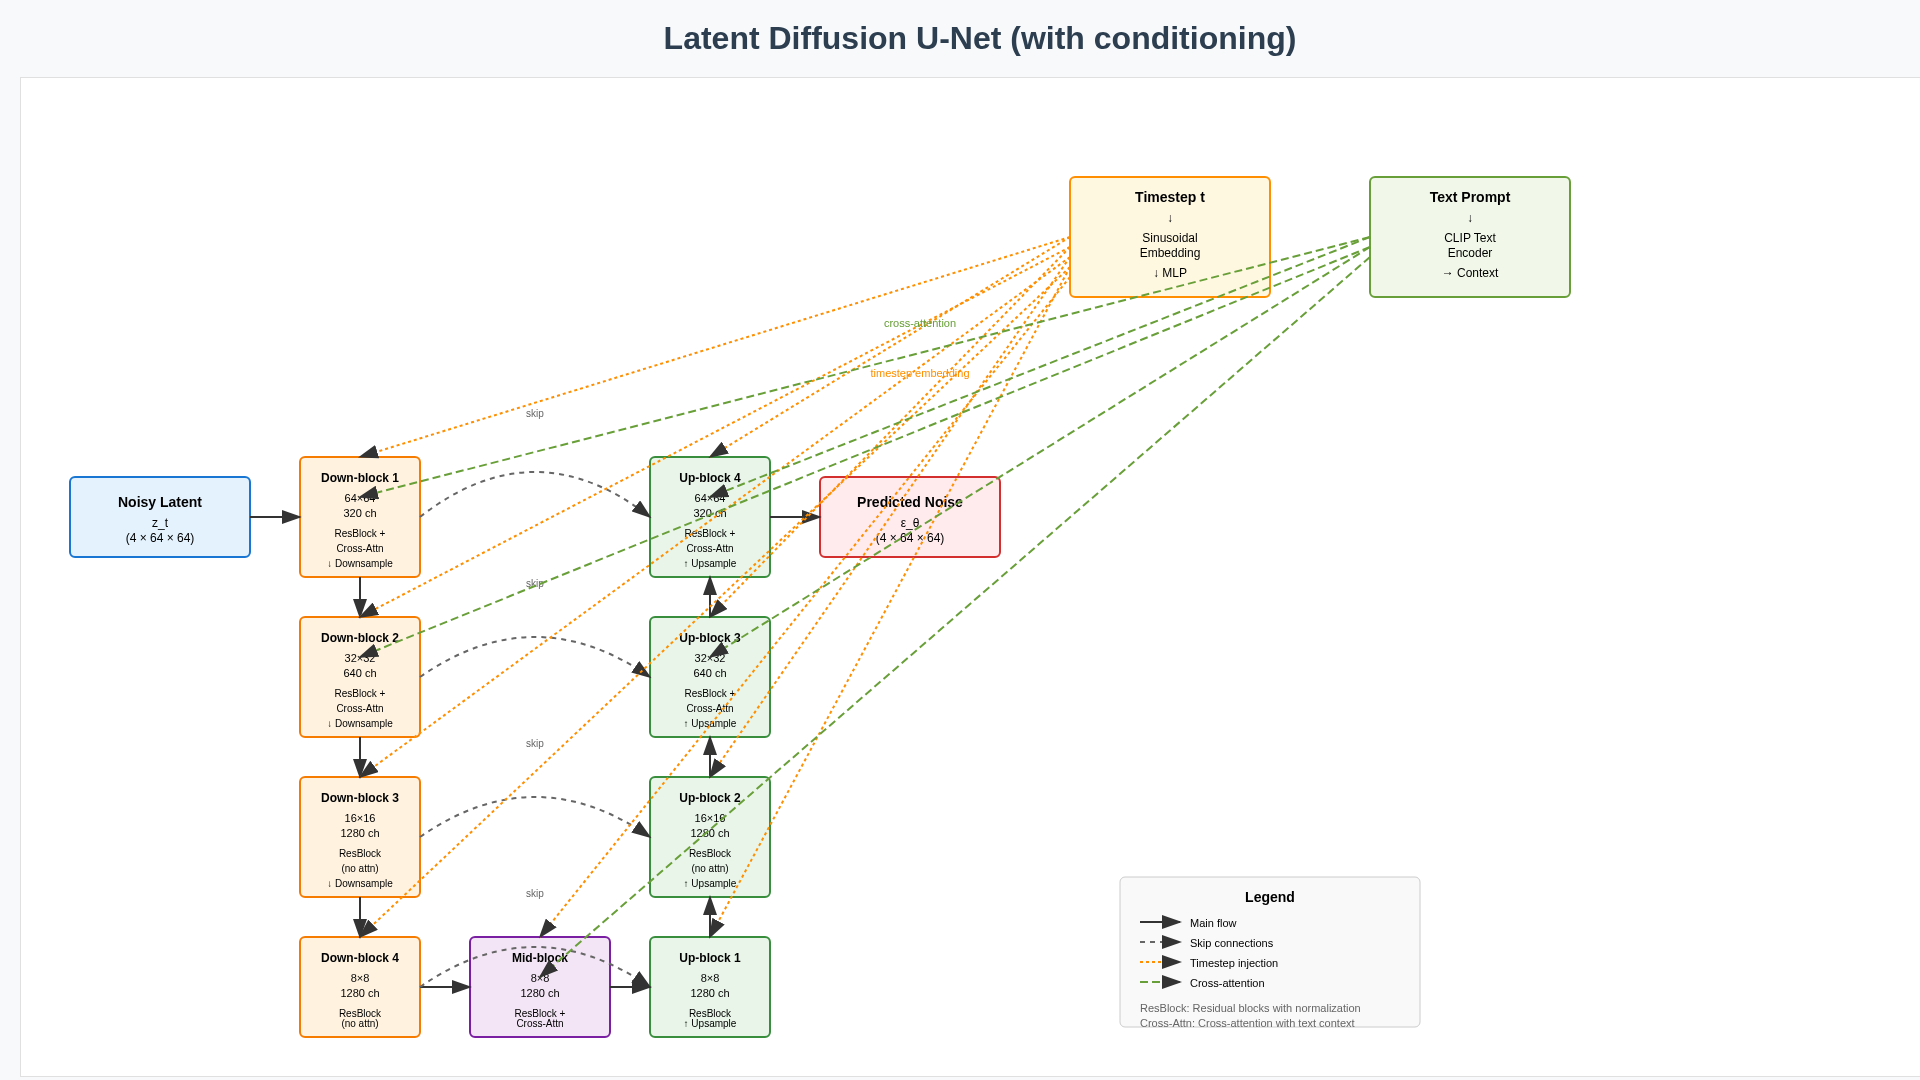
\includegraphics[width=\linewidth]{figures/diffusion_unet_singleshot.png}
\caption{\textbf{Single-shot.} Conditioning blocks crowd the down-block column, edges route through boxes and tangle at the center, and the legend collides with the decoder, all defects the geometry instrument flags but the VLM cannot see.}
\label{fig:ba-ss}
\end{subfigure}\hfill
\begin{subfigure}[b]{0.49\linewidth}
\centering
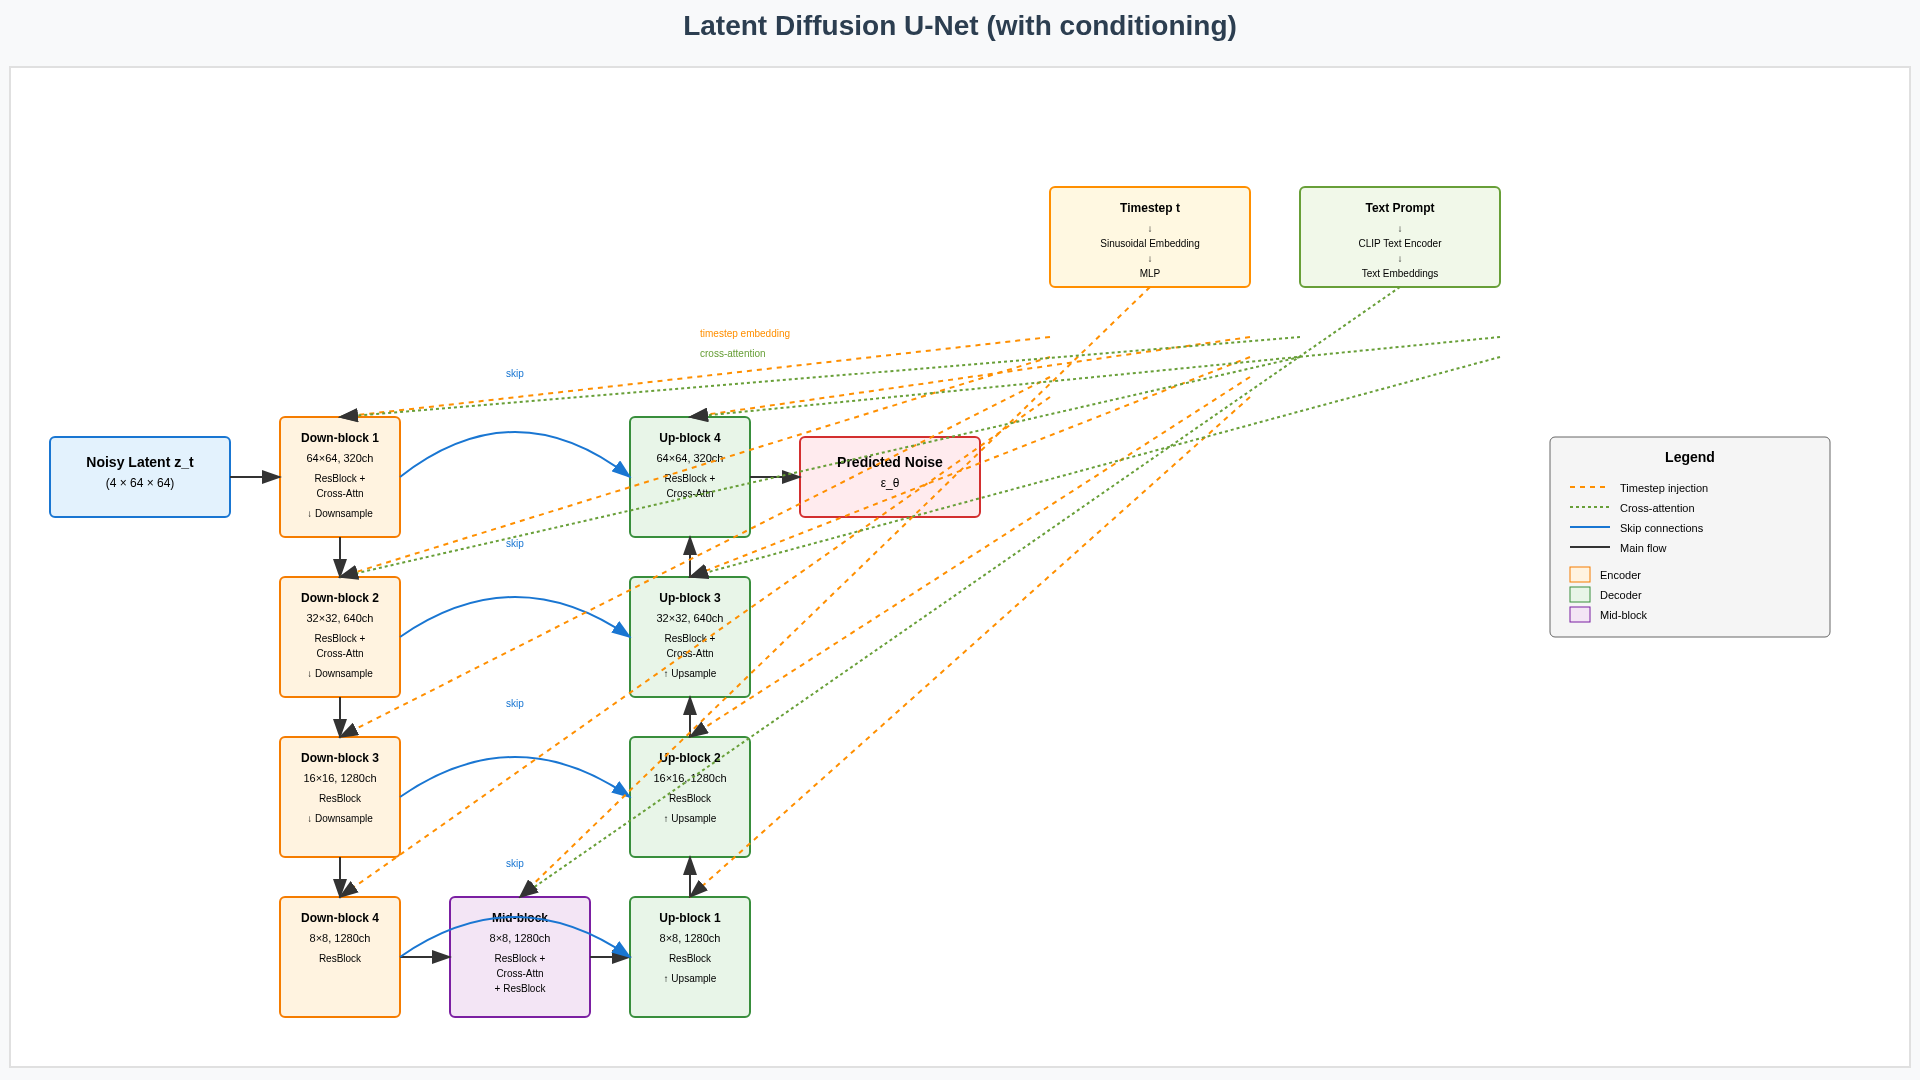
\includegraphics[width=\linewidth]{figures/diffusion_unet_reviewed.png}
\caption{\textbf{After grounded feedback.} The same task: conditioning blocks lifted clear, columns spaced and aligned, skip connections deconflicted, legend boxed in free space.}
\label{fig:ba-rv}
\end{subfigure}
\caption{\textbf{What grounded geometric feedback actually fixes.} The same academic-figure task, single-shot (\subref{fig:ba-ss}) vs.\ after the propose$\to$measure$\to$revise loop (\subref{fig:ba-rv}). This is the per-artifact reality behind the $-74\%$ mean defect reduction in \Cref{tab:geometric}, and exactly the difference a screenshot judge is blind to.}
\label{fig:beforeafter}
\end{figure}

\paragraph{A deterministic instrument reveals a large, significant effect across four modalities.} We score four visual modalities with the same DOM-geometry+alignment instrument under one identical configuration (Sonnet~4, temperature~$0$, design-principle prompt, three seeds, propose$\to$measure$\to$feed-exact-defects-back$\to$revise, $\le3$ iterations). \Cref{tab:geometric} and \Cref{fig:geomreduction} report the result: grounded geometric feedback produces a large, significant reduction in real layout defects on \emph{all four}, with bootstrap 95\% CIs that exclude zero and improvements sharply outnumbering regressions. The magnitudes track single-shot headroom: dense responsive web pages are defect-rich out of the box, while a frontier model under a design-principle prompt already lays out many figures and slides cleanly. Animations have the widest interval because their per-task defect counts are heavy-tailed across the dynamic suite, so we read the sign test as the robust statement and the mean as indicative.

\begin{table}[t]
\centering\small
\caption{Deterministic geometric-feedback results, one identical configuration across four visual modalities (Sonnet~4, $T{=}0$, $3$ seeds, alignment-inclusive reward). $\Delta$ is the mean defect reduction. CI is a paired bootstrap 95\% interval on $\Delta\%$ ($10$k resamples). $p$ is a two-sided paired sign test. Web is summed over $1920/375$ widths, animations over sampled frames.}
\label{tab:geometric}
\begin{tabular}{lcccccc}
\toprule
Modality & $n$ & SS & Rev. & $\Delta$ & 95\% CI & impr./regr.\ ($p$) \\
\midrule
Academic figures (20) & 60 & $0.57$ & $0.15$ & $-74\%$ & $[52,89]\%$ & $17/2$\;($7{\times}10^{-4}$) \\
Dense slides (12)     & 36 & $1.25$ & $0.33$ & $-73\%$ & $[45,93]\%$ & $13/1$\;($1.8{\times}10^{-3}$) \\
Web pages (20)        & 60 & $16.1$ & $8.5$  & $-47\%$ & $[30,62]\%$ & $33/2$\;($4{\times}10^{-8}$) \\
Animations (20)       & 60 & $16.9$ & $10.2$ & $-40\%$ & $[10,64]\%$ & $34/7$\;($3{\times}10^{-5}$) \\
\bottomrule
\end{tabular}
\end{table}

\begin{figure}[t]
\centering
\begin{tikzpicture}
\begin{axis}[width=0.86\linewidth,height=4.6cm,
  xbar,xmin=0,xmax=100,bar width=14pt,enlarge y limits=0.28,
  xlabel={geometric-defect reduction under grounded feedback (\%), bootstrap 95\% CI},
  symbolic y coords={Animations,Web pages,Dense slides,Academic figures},
  ytick=data,xtick={0,20,40,60,80,100},xmajorgrids]
  \addplot[draw=cRV!65!black,fill=cRV!55,
    error bars/.cd,x dir=both,x explicit,
    error bar style={cRV!60!black,line width=0.6pt},
    error mark options={cRV!60!black,mark size=2.4pt,line width=0.6pt}]
    coordinates {(74,Academic figures)+=(15,0)-=(22,0)
                 (73,Dense slides)+=(20,0)-=(28,0)
                 (47,Web pages)+=(15,0)-=(17,0)
                 (40,Animations)+=(24,0)-=(30,0)};
  % value labels at the bar base, clear of the CI whiskers
  \node[font=\footnotesize\bfseries,white,anchor=west] at (axis cs:1.8,Academic figures) {74\%};
  \node[font=\footnotesize\bfseries,white,anchor=west] at (axis cs:1.8,Dense slides) {73\%};
  \node[font=\footnotesize\bfseries,white,anchor=west] at (axis cs:1.8,Web pages) {47\%};
  \node[font=\footnotesize\bfseries,white,anchor=west] at (axis cs:1.8,Animations) {40\%};
\end{axis}
\end{tikzpicture}
\caption{\textbf{Grounded geometric feedback removes real layout defects on all four visual modalities} (mean reduction, with whiskers the paired-bootstrap 95\% CIs, all excluding zero). The standard VLM-on-a-screenshot metric measures none of this.}
\label{fig:geomreduction}
\end{figure}

\paragraph{An ungrounded \emph{reviewer} fails to fix layout, and on slides makes it worse (ablation, two modalities).} Grounding matters on the feedback side too. We fix the task suite and the proposer model and swap \emph{only} the reviewer's grounding. Because the two arms are separate runs, each is compared against its \emph{own} single-shot baseline, and single-shot geometry carries real seed-to-seed variance. So the load-bearing contrast is the \emph{direction} each reviewer moves its own baseline, not the absolute level (\Cref{fig:ablation}). The deterministic geometric-feedback reviewer sharply \emph{reduces} mean defects on both slides and figures, whereas the VLM-feedback reviewer does not: it increases defects on slides and is directionally worse on figures (not significant). Blind to the true geometry, its edits break alignment about as often as they fix it. On the same slides the binary VLM rubric simultaneously saturates, confirming the judge cannot even see the difference. Both halves of \Cref{fig:concept} are necessary.

\begin{figure}[t]
\centering
\begin{tikzpicture}
\begin{axis}[name=axslide,width=0.42\linewidth,height=3.9cm,ybar,bar width=10pt,
  ylabel={mean defects},title={\footnotesize slides},ymin=0,ymax=2.9,ytick={0,1,2},
  symbolic x coords={VLM-fb,geom-fb},xtick=data,enlarge x limits=0.6,
  nodes near coords,nodes near coords style={font=\scriptsize,/pgf/number format/.cd,fixed,precision=2},ymajorgrids]
  \addplot[draw=cGrey,fill=black!10] coordinates {(VLM-fb,1.89) (geom-fb,1.25)};
  \addplot[draw=cAccent!60!black,fill=cAccent!25] coordinates {(VLM-fb,2.44) (geom-fb,0.33)};
\end{axis}
\begin{axis}[at={($(axslide.east)+(1.4cm,0)$)},anchor=west,
  width=0.42\linewidth,height=3.9cm,ybar,bar width=10pt,
  title={\footnotesize academic figures},ymin=0,ymax=0.8,ytick={0,0.25,0.5},
  symbolic x coords={VLM-fb,geom-fb},xtick=data,enlarge x limits=0.6,
  nodes near coords,nodes near coords style={font=\scriptsize,/pgf/number format/.cd,fixed,precision=2},ymajorgrids,
  legend style={font=\footnotesize,at={(-0.14,1.26)},anchor=south,legend columns=2,draw=cGrey!50}]
  \addplot[draw=cGrey,fill=black!10] coordinates {(VLM-fb,0.52) (geom-fb,0.57)}; \addlegendentry{single-shot}
  \addplot[draw=cAccent!60!black,fill=cAccent!25] coordinates {(VLM-fb,0.62) (geom-fb,0.15)}; \addlegendentry{reviewed}
\end{axis}
\end{tikzpicture}
\caption{\textbf{An ungrounded reviewer fails to fix layout, while a grounded one does (controlled ablation, two modalities).} Same task suite and proposer model, with only the reviewer's grounding varying. The two arms are separate runs, so each is plotted against its \emph{own} single-shot (hence the differing single-shot bars). The VLM-feedback reviewer (\textsf{VLM-fb}) does not reduce defects and on slides increases them (slides $1.89\to2.44$, figures $0.52\to0.62$, directional/n.s.). The deterministic geometric-feedback reviewer (\textsf{geom-fb}) reduces them (slides $1.25\to0.33$, figures $0.57\to0.15$). The grounded signal is necessary on the feedback side, not just the metric side.}
\label{fig:ablation}
\end{figure}

\paragraph{Is the reduction circular?} The instrument both \emph{drives} the revision and \emph{scores} it, and the harness keeps the best-scoring iteration, so \emph{some} reduction is mechanically guaranteed. The honest questions are how large it is and whether it reflects quality a human would care about. Three facts argue it is not merely an artifact of optimizing the reported number. \textbf{(i)~The defects are real:} single-shot renders carry them at high rate (\Cref{fig:evoformer}), and the thresholds are deliberately conservative ($\ge6$\,px overlap, $>16$\,px overflow), so a flagged defect is visible, not sub-perceptual. \textbf{(ii)~The magnitude is not preordained:} keeping the best of three iterations could in principle move the metric by almost nothing. That grounded revision instead removes a large fraction of real defects (\Cref{tab:geometric}) is a property of the feedback, not the keep-best rule. \textbf{(iii)~The ungrounded-reviewer ablation is the decisive control:} scored by the \emph{same} metric, the VLM-feedback arm \emph{fails} to reduce it (and worsens slides). So the reduction tracks the \emph{grounding} of the feedback, not the act of optimizing the scorer, a conclusion the model-free cross-model replication (\Cref{sec:robustness}) reinforces. What remains open, and is the principal caveat of the geometric measurement, is a quantitative human-preference study confirming that DOM-defect reduction maps onto perceived-quality gains across the full suite.

\paragraph{Two modalities where the honest answer is ``no headroom.''} \emph{Video editing}, scored by Gemini~3.1~Pro's native full-clip rubric (a near-grounded instrument that observes pixels, not a still), is already strong single-shot, so the reviewed lift is small and not significant. A hardened multi-step suite de-saturates it. \emph{Deep research}, scored against exact provided facts, saturates: a frontier model knows well-documented facts and does not take the planted traps, so the Type-3d lift is bounded by the near-zero single-shot error rate. This is a genuine limit of the factual modality, since de-saturating it would require facts the judge itself cannot grade. We report these as scoped negatives rather than headline lifts (\Cref{tab:harness-headline}).
